\documentclass[11pt,a4paper]{article}
\usepackage[T1]{fontenc}
\usepackage[utf8]{inputenc}
\usepackage{lmodern,microtype}
\usepackage[a4paper,margin=24mm,headheight=15pt]{geometry}
\usepackage{amsmath,amssymb,graphicx,booktabs,array}
\usepackage{xcolor,enumitem,fancyhdr}
% Selected definitions imported from the ITACA manuscript on 2026-10-22.
% Source: /Users/jjgomezcadenas/Papers/itaca/pool/NextDefs.tex
% Used by itacaRevisited.tex alongside pool/NextLatexPackagesBase.tex.
% Local copy: compiling this note does not require the external directory.
% Preserve source macro names and notation; omit numerical design inputs,
% run-specific measurements, draft labels and conflicting SI unit aliases.
\usepackage{siunitx,xspace}
\sisetup{separate-uncertainty=true}

% Double-beta decay
\newcommand{\bb}{\ensuremath{\beta\beta}}
\newcommand{\bbonu}{\ensuremath{\beta\beta0\nu}}
\newcommand{\bbtnu}{\ensuremath{\beta\beta2\nu}}
\newcommand{\Qbb}{\ensuremath{Q_{\beta\beta}}}
\newcommand{\mbb}{\ensuremath{m_{\beta\beta}}}
\newcommand{\Tonu}{\ensuremath{T_{1/2}^{0\nu}}}
\newcommand{\Ttnu}{\ensuremath{T_{1/2}^{2\nu}}}
\newcommand{\Monu}{\ensuremath{\Big|M_{0\nu}\Big|}}
\newcommand{\Mtnu}{\ensuremath{\Big|M_{2\nu}\Big|}}
\newcommand{\Gonu}{\ensuremath{G_{0\nu}(\Qbb, Z)}}
\newcommand{\Gtnu}{\ensuremath{G_{2\nu}(\Qbb, Z)}}

% Isotopes and ion species
\newcommand{\XE}{\ensuremath{{}^{136}\rm Xe}}
\newcommand{\XEO}{\ensuremath{^{137}}Xe}
\newcommand{\BI}{\ensuremath{{}^{214}\rm Bi}}
\newcommand{\TL}{\ensuremath{{}^{208}\rm{Tl}}}
\newcommand{\KR}{\ensuremath{^{83m}\mathrm{Kr}}\xspace}
\newcommand{\Xe}[1]{\ensuremath{^{#1}\mathrm{Xe}}\xspace}
\newcommand{\Bi}[1]{\ensuremath{^{#1}\mathrm{Bi}}\xspace}
\newcommand{\Tl}[1]{\ensuremath{^{#1}\mathrm{Tl}}\xspace}
\newcommand{\Kr}[1]{\ensuremath{^{#1}\mathrm{Kr}}\xspace}
\newcommand{\xetp}{\ensuremath{{\rm Xe_2^{+}}}}
\newcommand{\batp}{\ensuremath{{\rm Ba^{2+}}}}
\newcommand{\nhfp}{\ensuremath{{\rm NH_4^{+}}}}
\newcommand{\nht}{\ensuremath{{\rm NH_3}}}

% Detector names and terminology
\newcommand{\NEW}{NEXT-White}
\newcommand{\NEXT}{NEXT-100}
\newcommand{\GXeEL}{GXeEL}
\newcommand{\HPXe}{HPXe}
\newcommand{\HPXeEL}{HPXe-EL}
\newcommand{\TM}{\emph{Topmetal}\xspace}

% Signals, transport and statistical notation
\newcommand{\tz}{\ensuremath{t_0}}
\newcommand{\sone}{\ensuremath{S_1}}
\newcommand{\stwo}{\ensuremath{S_2}}
\newcommand{\nph}{\ensuremath{n_\gamma}}
\newcommand{\VDR}{\ensuremath{v_d}}
\newcommand{\VD}{\ensuremath{v_d}}
\newcommand{\REF}{\ensuremath{\frac{E}{P}}}
\newcommand{\REY}{\ensuremath{\frac{Y}{P}}}
\newcommand{\chitwo}{\ensuremath{\chi^2}}
\newcommand{\SigmaE}{\ensuremath{\sigma_E / E}}
\newcommand{\stat}{\textrm{(stat.)}}
\newcommand{\sys}{\textrm{(sys.)}}

% Reference and table helpers
\newcommand{\fig}{figure}
\newcommand{\eq}{equation}
\newcommand{\tab}{table}
\newcommand{\Fig}{Figure}
\newcommand{\Eq}{Equation}
\newcommand{\Tab}{Table}
\newcommand{\minitab}[2][l]{\begin{tabular}{#1}#2\end{tabular}}

\usepackage[numbers,sort&compress]{natbib}
\usepackage[colorlinks=true,linkcolor=blue!45!black,citecolor=blue!45!black,urlcolor=blue!45!black]{hyperref}
\graphicspath{{generated/}}
\setlength{\parindent}{0pt}
\setlength{\parskip}{5pt plus 1pt}
\setlength{\emergencystretch}{2em}
\setlist{nosep,leftmargin=*}
\pagestyle{fancy}
\fancyhf{}
\fancyhead[L]{\small NAUSICA for ITACA}
\fancyhead[R]{\small \today}
\fancyfoot[C]{\thepage}
% Generated by scripts/benchmarks/build_physics.py; do not edit.
\newcommand{\OpenFraction}{0.04909}
\newcommand{\EntranceThreshold}{4.074}
\newcommand{\FluxRatio}{1.227}
\newcommand{\Mobility}{5}
\newcommand{\DiffusionCoefficient}{1.263}
\newcommand{\PeakCurrent}{1.731}
\newcommand{\DiskPeakCurrent}{1.923}
\newcommand{\FinalNinetyTime}{193.51}
\newcommand{\GapChargeFraction}{0.9984124}
\newcommand{\GapPotential}{0.0015876}
\newcommand{\GapMissingPercent}{0.1588}
\newcommand{\SquareHalfWidth}{0.25}
\newcommand{\GapSpeed}{3}
\newcommand{\ConfigHash}{628be0c9c8b9}

\newcommand{\ion}{\ensuremath{\mathrm{Xe}_2^+}}
\newcommand{\dd}{\mathrm{d}}
\title{NAUSICAA for ITACA}
\author{J. J. G\'omez-Cadenas}
\date{\today}

\begin{document}
\maketitle
\thispagestyle{fancy}
\begin{abstract}
ITACA (Ion Tracking Apparatus with CMOS ASICs) is a proposed new detector to search for neutrinoless double beta decay (\bbonu) events in a future, (multi) ton scale, ultra-low background, high pressure xenon TPC. The crucial innovation introduced by ITACA is the measurement of both the electron and the ion tracks produced in the xenon gas in response to ionizing particles. The readout of the ion track involves the use of electronics able to measure the charge carried by the positive xenon ions arriving at the cathode. We propose a design based on bare metal pads (TopMetal) coupled to CMOS electronics, which we call NAUSICA (Non-Amplified Ultra-Slow Ion CMOS ASIC). 

This paper presents a conceptual design of NAUSICA and a simplified model of its response to ion tracks. We use a Geant4-based simulation of ITACA to generate \bbonu\ events uniformly in the fiducial volume of the detector. The ions produced by each track drift to the cathode where they are focused towards the metal electrodes. We calculate the distribution of ion arrival positions and times after drift, diffusion and focusing and the current induced on each collection pad. A charge-sensitive amplifier (CSA) computes the voltage produced as this current is integrated on a feedback capacitor with a finite discharge time. We then add electronic noise and digitise the voltage to obtain the digitised signal from each pad. The combined response of all the pads with signals above a noise-dependent threshold allows the reconstruction of the track. We show that the track can be
resolved above the noise, keeping its characteristic topology.

\end{abstract}

\section{Introduction}

The next generation of neutrinoless double-beta decay (\bbonu) experiments, aiming to establish if the neutrino is its own antiparticle, will attempt to explore lifetimes for a putative decay, $T_{1/2} > 10^{28}$~yr. This ambitious goal will require (multi) ton target masses of a double-beta decaying isotope and essentially zero backgrounds~\cite{Gomez-Cadenas:2023vca}. 
High Pressure Xenon TPCs (HPXe)~\cite{Gomez-Cadenas:2019ges} are one of the leading technologies for such a generation of large, virtually background-free \bbonu\ detectors. In particular, the NEXT collaboration is currently operating the NEXT-100 apparatus \cite{NEXT:2025yqw} at the Canfranc Underground Laboratory, a large scale detector which can hold $\sim100$~kg of xenon at 15~bar, in a high pressure time projection chamber of roughly 1~m$^3$ volume. NEXT has already demonstrated a FWHM energy resolution of $(0.93 \pm 0.02)$\% at \Qbb~\cite{NEXT:2025ozn}. 

An HPXe TPC provides a distinctive topological signature that enables identification of events with two emitted electrons. A \bbonu\ candidate is defined as a single, continuous track, with no detached energy deposits and fully contained inside the fiducial volume. The energy of the track must be close to \Qbb\, typically within a ROI of $\pm 1\sigma$.  This ``single-track'' requirement suppresses nearly all backgrounds, leaving only single-electron events with energies near \Qbb, such as those arising from photoelectric interactions (without an accompanying X-ray satellite) of the 2.448~MeV $\gamma$ ray of \BI\ and the 2.615~MeV $\gamma$ ray of \TL, as well as from beta decays of $^{137}$Xe created by cosmogenic activation. In addition, requiring large local energy deposits (``blobs'') near the two endpoints of the track permits an additional suppression of single electron backgrounds that make it into the ROI. The effectiveness of this topological discrimination has been demonstrated by the NEXT collaboration~\cite{Ferrario:2015kta, Ferrario:2019kwg, NEXT:2021vzd, Kekic2021, NEXT:2021pjq}. 

However, the performance of the topological signature in an HPXeEL TPC is limited by diffusion and by electroluminescent blurring. As ionisation electrons drift through the dense gas, they undergo diffusion, producing a charge cloud whose transverse size increases with the drift length. In addition, EL amplification introduces further smearing, as the EL photons are emitted isotropically. 

In two recent papers~\cite{Gomez-Cadenas:2025ect, itaca2026}, we proposed a new approach to improving the topological signature, while preserving EL amplification, needed for energy resolution. The method relies on recording two complementary tracks for each event: the \emph{electron track}---the established signature in an HPXeEL TPC---and the \emph{ion track}, formed by the positive ions left along the original particle trajectory. The ion track exhibits diffusion at the millimetre level and is free from EL-induced smearing, providing a dramatic boost to topological discrimination.
The Ion Tracking Apparatus with CMOS ASICs (\textsc{ITACA})~\cite{itaca2026} is a proposed high pressure xenon TPC based on this principle. The ions are read out using bare metal pads (TopMetal) coupled to CMOS electronics.

In this paper we present a conceptual design of NAUSICA (Non-Amplified Ultra-Slow Ion CMOS ASIC), our proposed readout for ITACA. Our study~\cite{itaca2026} showed that the topological signature that allows distinguishing between signal (\bbonu\ events which produce two electrons) and single-electron backgrounds could increase the rejection power of the HPXe technology by at least one order of magnitude, provided that the ion track could be reconstructed with a spatial resolution at the level of
ion diffusion ($\sigma \sim 1$--$2$~mm). Here we show that the proposed NAUSICA readout can preserve the resolution at the level dictated by the diffusion, thus guaranteeing the expected enhancement of the topology discrimination power.

This paper is organized as follows. Section \ref{sec:itaca_det} briefly summarizes the main aspects of the ITACA detector. 
Section \ref{sec:nausica} presents the NAUSICA concept.
% TODO: Complete the roadmap after the new sections are in place.


\section{The ITACA Detector}
\label{sec:itaca_det}

The pressure of operation in ITACA is chosen as a tradeoff between mass --- which increases with pressure --- and track topology, which is easier to resolve at lower pressure. Other considerations include ion drift velocity, which decreases approximately inversely with pressure at fixed electric field, and electron lifetime, which tends to improve at lower pressure. Overall, 15 bar is a good compromise. Using electroluminescence to amplify the electron track signal guarantees excellent energy resolution. Fiducialisation of the event requires the measurement of $t_0$, provided by primary scintillation. Both requirements are essential for a \bbonu\ experiment.
 
 \begin{figure}[!htbp]
    \centering
    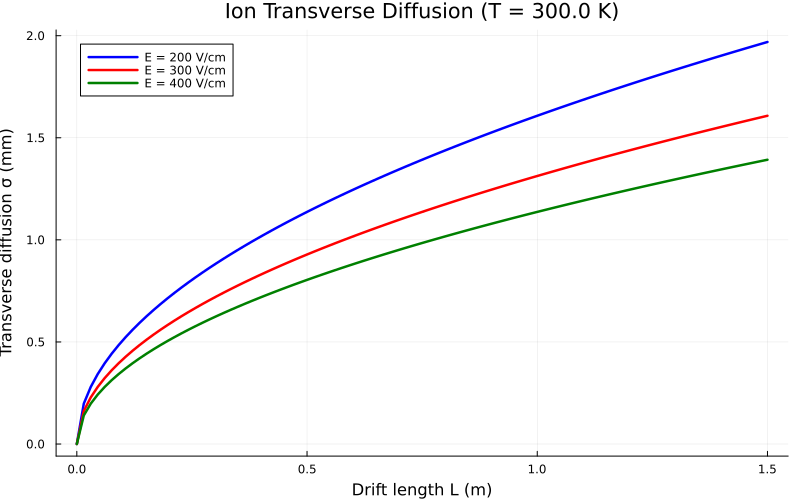
\includegraphics[scale=0.25]{img/ion_diffusion_vs_length.png}
     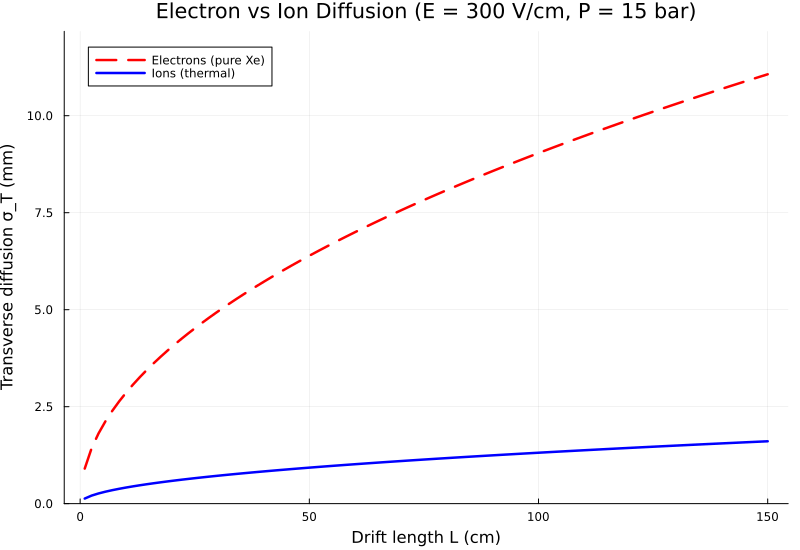
\includegraphics[scale=0.25]{img/electron_ion_diffusion.png}
    \caption{Left: transverse diffusion of \xetp\ ions as a function of drift length for three different drift fields; right: transverse diffusion of \xetp\ ions compared with transverse diffusion of electrons in pure xenon.}
    \label{fig:sigmatvsl}
\end{figure}
 
 
\begin{table}[htbp]
\centering
\caption{Summary of ITACA detector parameters.}
\label{tab:itaca_params}
\begin{tabular}{@{}llrl@{}}
\toprule
\textbf{Parameter} & \textbf{Symbol} & \textbf{Value} & \textbf{Unit} \\
\midrule
\multicolumn{4}{@{}l}{\textit{Geometry}} \\
Fiducial diameter      & $D_{\mathrm{fid}}$   & 320   & cm \\
Fiducial height        & $L_{\mathrm{fid}}$   & 150   & cm \\
Fiducial volume        & $V_{\mathrm{fid}}$   & 12.1  & m$^3$ \\
Fiducial Xe mass       &                      & 1050  & kg \\
PV internal diameter   &                      & 3.54  & m \\
PV internal height     &                      & 2.01  & m \\
\midrule
\multicolumn{4}{@{}l}{\textit{Electric field and drift}} \\
Drift field            & $E$                  & 200   & V/cm \\
Electron drift velocity& $v_e$                & 1     & mm/$\mu$s \\
Electron drift time    & $t_e$                & 1.5   & ms \\
Ion drift velocity     & $v_d$                & 10    & cm/s \\
Ion drift time (max)   & $t_{\mathrm{max}}$   & 15    & s \\
\bottomrule
\end{tabular}
\end{table}


 Choosing the detector dimensions implies a tradeoff between the diameter and the length of the TPC. A major design goal is to minimise the transverse diffusion $\sigma_T$ of ions, which in the thermal limit is simply:
 %
 \begin{equation}
\sigma_T =\sqrt{\tfrac{2k_BT}{q_e}\tfrac{L}{E}} 
\label{eq:drift}
\end{equation}
%
where $L$ is the ion drift distance, $E$ the drift field, $T$ the gas temperature, $k_B$ Boltzmann's constant and $q_e$ the elementary charge. Equation~\ref{eq:drift} favours shorter $L$ and larger $E$. Figure~\ref{fig:sigmatvsl} shows $\sigma_T$ for three different drift fields. For a TPC drift length of 150~cm, the average $\sigma_T$ is of the order of \SI{1}{mm}, one order of magnitude smaller than the corresponding diffusion for electrons in pure xenon.

Another important design factor is the voltages in the TPC electrodes. All sensors (the CMOS reading the ions and the SiPMs reading the EL light) operate best at ground, but the drifting of electrons and ions requires a constant field in the TPC, and the generation of EL light requires an additional, higher field, in the EL region. 

The cathode is instrumented with an Ion Focusing Grid (IFG) which focuses the incoming ions into the readout pads of the CMOS detector. The upper electrode of the IFG is at a voltage $V_c = \SI{8}{kV}$. The voltage on the anode side of the TPC depends on the drift length and the drift field. A good compromise between minimising diffusion and keeping voltage at the anode reasonable is to choose a drift field of \SI{200}{V/cm}, which results in \SI{38}{kV} at the first anode electrode, and \SI{54}{kV} at the second (with \SI{16}{kV} across the EL gap). 
 
 Once the length of the TPC is defined, the diameter of the TPC defines the fiducial mass that can be achieved. At 15 bar, choosing $D= 320$ cm, results in a fiducial mass slightly above one ton, $M_{fid} = 1050$ kg. 
 
 A large diameter TPC requires instrumenting both the EL side (with SiPMs) and the cathode side (with top metal devices). 
  Previous work involving the detection of
 ions for \bbonu\ experiments \cite{Nygren_2018, mei2020topmetalcmosdirectcharge} has quantified the challenge of instrumenting a large surface with CMOS detectors, which appears, nonetheless, feasible \cite{You2021}. The ITACA paper~\cite{itaca2026} proposes a movable ion detector, the Magnetically Actuated Rotor System (MARS). The NAUSICA readout considered here could be used as part of MARS or to instrument the full cathode.  Table~\ref{tab:itaca_params} shows the main parameters of a 1-ton ITACA detector. 

% =================================================================
\subsection{Principle of operation}
\label{sec:pof}

Consider a putative \bbonu\ event occurring in the middle of the TPC. Two electrons, with a total energy of \Qbb\ (\SI{2458}{keV}), propagate through the dense noble gas, ionising it. Primary scintillation is recorded and a fast trigger system (FTS) records the start-of-the-event $t_0$. Then a fast measurement of the event energy is performed, accepting the event only if its energy lies within a pre-determined ROI (selected to be $\pm 1\sigma$ around \Qbb). Events outside the ROI are rejected and no ion readout is attempted.

Since the event that we are considering is a \bbonu\ decay, the FTS will likely trigger, activating a fast reconstruction of the topology and event barycenter, $(x_i, y_i, z_i)$. The coordinates $(x_i,y_i)$ predict the landing position of the ion cloud at the cathode, while $z_i$, together with $t_0$ and the ion drift velocity, determines the arrival time of its barycenter ($t_i$). 

     
The \xetp\ ions reach the cathode on a time scale of seconds. In our specific example, with the event at the midpoint of the TPC, they need to drift \SI{75}{cm} at a velocity of \SI{10}{cm/s}, requiring \SI{7.5}{s}. 
The typical longitudinal extension of the ion track is of the order of \SI{10}{cm}, and thus about \SI{1}{s} is needed to collect the ions. 

Notice that the electron track and the ion track are detected in \emph{delayed coincidence}. The ion track is intercepted precisely at the right time and in the right place, thus minimising the impact of spurious coincidences. At the expected trigger rate (dominated by backgrounds in the ROI), pile-up during the $\sim$\SI{15}{s} maximum ion drift time is negligible.


\section{The NAUSICA concept}
\label{sec:nausica}

Reading the arriving ions (without amplification) requires exposed metal electrodes connected to charge-sensitive amplifiers (CSAs). Our proposed  \emph{Non-Amplified Ultra-Slow Ion CMOS ASIC} (NAUSICA) uses TopMetal CMOS technology~\cite{An2016TopmetalII} to implement this concept, following Refs.~\cite{Nygren_2018, mei2020topmetalcmosdirectcharge}. There is an important difference, however, with respect to these works, which attempted to design a system able to provide simultaneously good energy resolution and a good measurement of the track topology using ions. Alas, both requirements impose constraints that interfere with each other. Good energy resolution requires optimizing ion counting and minimizing noise. Good topological reconstruction demands pixels separated by a small pitch (e.g., of the order of diffusion, $\sim 2$ mm), which in turn multiplies the number of pixels and adds to the overall noise. The advantage of ITACA is that energy resolution is measured with excellent precision by electroluminescence, and thus the ion detector can prioritize the reconstruction of the topology. NAUSICA is designed with this goal in mind. 

The principle of operation is as follows. The ions arrive at the metal pad over a time of order 1 second, taking a 10 cm extent along the drift direction as an extreme case. The resolution in $z$ should be of the order of the resolution in the transverse coordinates ($\sigma_z = 1-2$ mm). Since the drift velocity of the ions is $\sim 10$ cm/s, this translates into slicing the charge in buckets of $10-20$ ms, which implies a framed readout (about 50 frames of 20 ms each). The mean number of ions per pad in those buckets helps determine the feedback capacitance of the CSA. The sampled voltage includes charge accumulated in previous buckets. The charge arriving in each bucket is recovered from the change between successive samples, accounting for feedback discharge. 


\begin{figure}[!htbp]
    \centering
    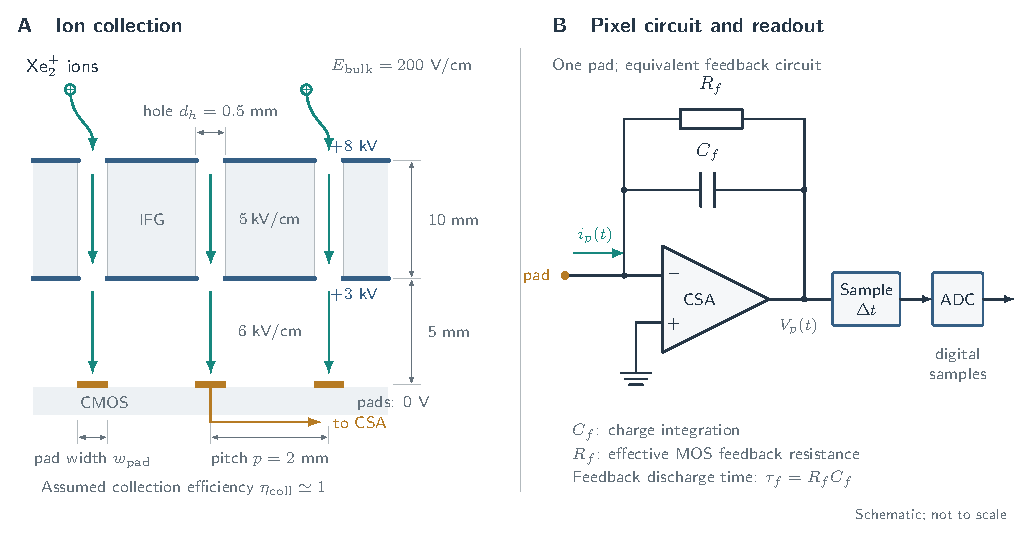
\includegraphics[width=\linewidth]{figures/nausica_concept.pdf}
    \caption{NAUSICA ion collection geometry (left) and equivalent pixel circuit (right). The drawing is schematic and not to scale.}
    \label{fig:nausicaa}
\end{figure}


\subsection{Charge collection and focusing}

The pad dimensions and pitch need to be chosen balancing the desired spatial resolution with the need for an acceptable signal-to-noise (S/N) per pad. Larger pads increase the collection but also the input capacitance, thus the need to focus the incoming ions in an area as small as possible. The left panel of Fig. \ref{fig:nausicaa} shows a schematic of the Ion Focusing Grid (IFG), which does this job.  We estimate the focusing requirement by comparing the electric flux through one pixel cell with that through its hole. Taking uniform fields in the drift region and inside the hole, full flux collection requires
\[
E_h\,\frac{\pi d_h^2}{4}\gtrsim E_{\rm bulk}p^2.
\]
Here $E_h$ and $E_{\rm bulk}$ are the fields inside the hole and in the drift region, respectively, $d_h$ is the hole diameter, and $p$ is the pixel pitch.
For a pitch of 2 mm, a bulk field of 200 V/cm and a hole field of 5 kV/cm, this gives a minimum hole diameter of approximately 0.45 mm. Thus, we take 0.5 mm as a preliminary design parameter. Full flux collection in this simple geometry implies a large ion collection efficiency that we take as one for the time being.  The validity of this approach is shown in Appendix B.





\subsection{Pixel electronics and readout}

Each pad is directly connected to the input of a CSA. The input current is integrated on a feedback capacitor, while a MOS pseudo-resistor operating in the subthreshold regime provides continuous discharge. The feedback capacitance sets the charge-to-voltage gain, and the discharge time determines how long the accumulated signal is retained.

Ion charge collection is continuous in time. The detector is read out using a frame-based scan of the pixels. Digitisation is performed at the periphery of the ASIC or on an external carrier, using one or a small number of multiplexed ADCs. The pad positions and the time dependence of their signals provide the three-dimensional ion image, using the known ion drift velocity to reconstruct the longitudinal coordinate.

\subsection{Parameters of the design}

The pad size, pitch and active area must be chosen to sample and contain the ion track. The feedback capacitance and discharge time depend on the charge arriving at each pad and its distribution in time. The sampling interval, electronic noise and ADC range must allow the weaker parts of the track to be recorded while accommodating the largest signals.

To specify these parameters, we first calculate the current induced by one ion and the resulting CSA voltage. We then calculate the distribution of charge among pads and its arrival times for simulated tracks. These calculations determine the readout parameters, which are finally tested by reconstructing tracks with electronic noise and digitisation included.

% BEGIN ORIGINAL SECTION 3 -- retained for author review and redistribution
% Track distributions belong in planned Section 5; design specifications in Section 6.
% \section{NAUSICA for ITACA}
% \label{sec:nausica}
% \begin{figure}[!htbp]
%     \centering
%     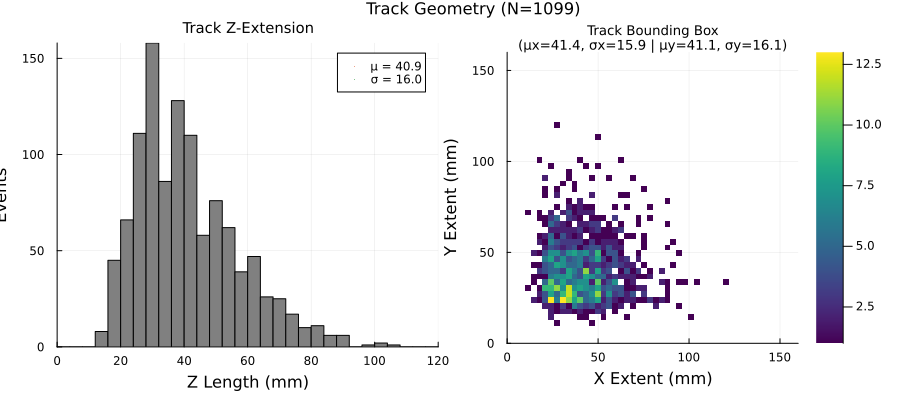
\includegraphics[scale=0.40]{img/z_xy_extent.png}
%     \caption{Left panel: z extension of \bbonu\ events; right panel: bounding box (maximum extension in x-y) of \bbonu\ events }
%     \label{fig:zoc}
% \end{figure}
% 
% \begin{figure}[!htbp]
%     \centering
%     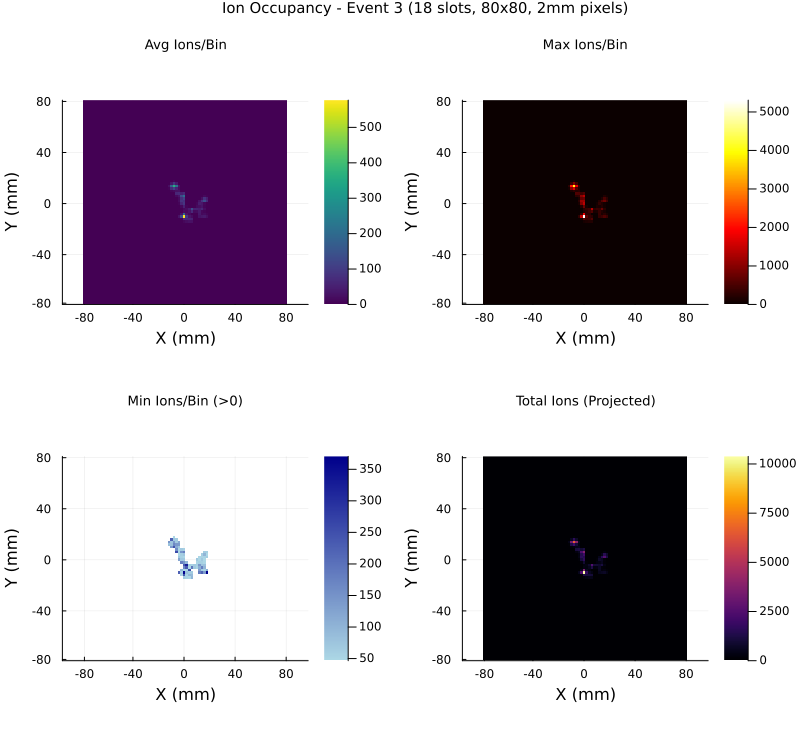
\includegraphics[scale=0.40]{img/occupancy_heatmaps.png}
%     \caption{Typical occupancy heatmaps for \bbonu\ events, showing the spatial distribution of ion hits across the pixel plane for representative simulated decays.}
%     \label{fig:oc2d}
% \end{figure}
% 
% 
% The key requirements for a detector designed to record the ions, are:
% \begin{enumerate}
% \item {\bf Containment of the track in XY}, requires an active area of $\mathrm{160 \times 160\ mm^2}$. 
% \item{\bf Sample of the track along Z}, requires sampling the track every \SI{10}{ms} over \SI{1}{s}
% \item{\bf Resolution along XY}, depends on diffusion and pitch ($p$) between pixels. Choosing $\mathrm{p = 2\ mm}$,  provides a resolution of
% $ \sigma_{\mathrm{p}} = \frac{p}{\sqrt{12}} \simeq 0.58~\mathrm{mm}$, which conveniently oversamples diffusion. 
% \item{\bf Resolution along Z}, sampling every \SI{10}{ms}, provides a Z resolution of 
% \SI{1}{mm}, matching the diffusion. 
% \item{\bf Photon-track separation} is defined by the pitch. A minimum separation of 
% \SI{2}{mm} maximises the compromise between acceptable signal efficiency and background rejection, given the ion diffusion. 
% \end{enumerate}
% 
% \subsection{Direct ion imaging with CMOS Topmetal sensors}
% 
% Direct collection of drifting ions on a segmented charge-sensitive plane, as proposed in 
% \cite{Nygren_2018, mei2020topmetalcmosdirectcharge}
%  is a natural solution in this regime. CMOS Topmetal sensors provide exposed metal electrodes directly connected to per-pixel charge-sensitive amplifiers (CSAs), enabling long integration times and frame-based readout well matched to slow ion drift.
% 
% The Topmetal II sensor~\cite{An2016TopmetalII} established the basic architecture for direct
% charge collection using CMOS technology. Each pixel integrates an exposed metal pad, a CSA
% with femtofarad-scale feedback capacitance, and a frame-based readout scheme. This work
% demonstrated that sub-100~$e^{-}$ equivalent noise charge can be achieved for direct charge
% sensing, providing the technological foundation for subsequent developments.
% 
% 
% \subsection{The NAUSICA concept}
% 
% \begin{figure}[!htbp]
%     \centering
%     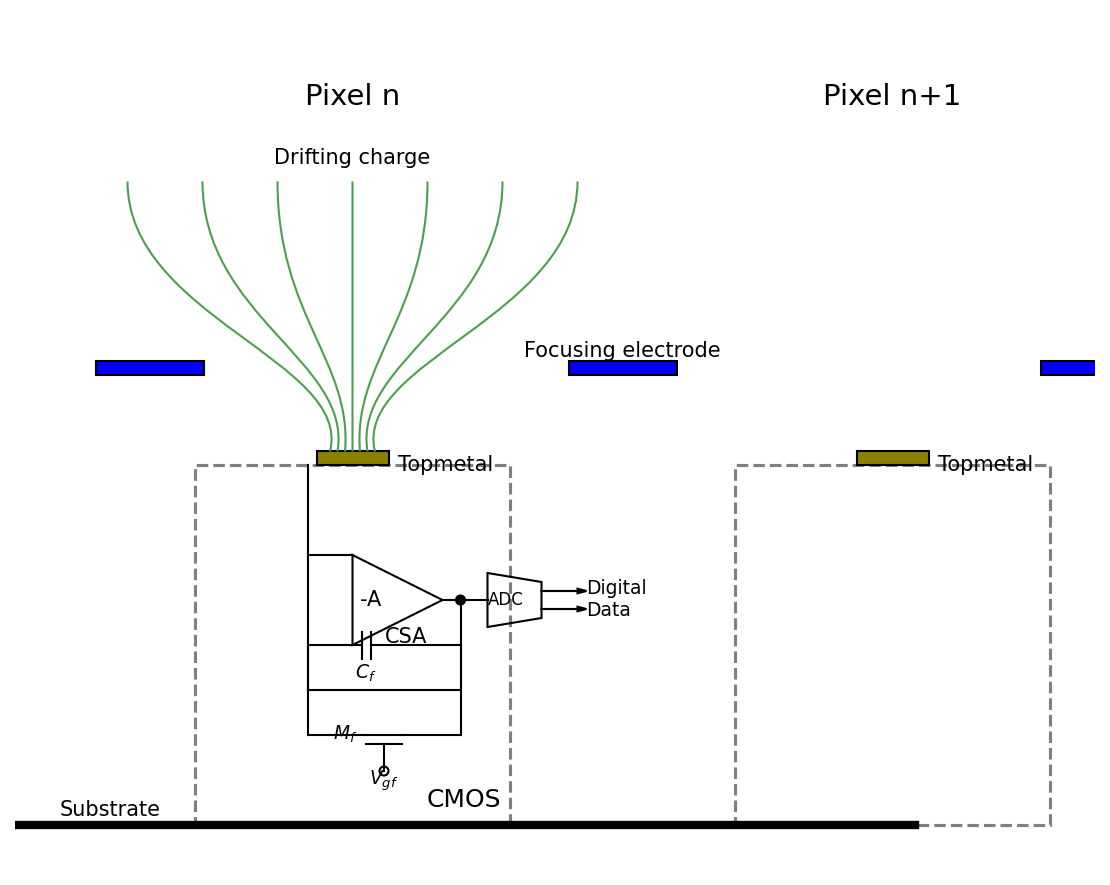
\includegraphics[scale=0.80]{img/topmetal_diagram.png}
%     \caption{Sketch of the NAUSICA concept (adapted from \cite{Nygren_2018}). An bare electrode in the topmost layer of CMOS (Topmetal, shown as a yellow rectangle) collects charge in gas directly. Internal
% Charge Sensitive Amplifier (CSA) converts charge signal into voltage waveform, which is then digitized by the integrated ADC (located in the periphery). Digital signals are transmitted off the chip. An elevated and separately biased electrode (blue rectangles) creates a focusing electrostatic field between itself and the Topmetal electrode (green curves).}
%     \label{fig:nausicaa}
% \end{figure}
% 
% The Topmetal-based sensor for ITACA, is named
% \textbf{NAUSICA} (Non-Amplified Ultra-Slow Ion CMOS ASIC. It is implemented in a 180~nm mixed-signal CMOS technology (Figure~\ref{fig:nausicaa}) with the following specifications.
% 
% \subsubsection*{Charge collection pads and focusing}
% 
% Each pixel includes an exposed metal charge-collection pad with dimensions
% $    A_{\mathrm{pad}} = 0.5 \times 0.5~\mathrm{mm^2}.$
% The pad size is chosen to minimise input
% capacitance and electronic noise. Efficient charge collection across the full pixel cell
% is ensured by electrostatic focusing electrodes.
% 
% \subsubsection*{Readout mode and temporal sampling}
% 
% Ion charge collection is continuous in time. The longitudinal coordinate is reconstructed
% from time sampling, using the known ion drift velocity. To achieve a longitudinal resolution
% of order 1~mm, the sensor is read out in frames with a period
% $
%     \Delta t = 10~\mathrm{ms},
% $
% corresponding to a frame rate of 100~Hz. The full ion track is therefore sampled over
% approximately 100 frames.
% 
% \subsubsection*{Pixel-level analogue front-end}
% 
% Each pixel implements a minimal analogue front-end optimised for slow signals:
% \begin{itemize}
%     \item An exposed metal pad directly connected to the input of a charge-sensitive
%     amplifier (CSA).
%     \item A feedback capacitor with nominal value
%     $C_f \simeq 5~\mathrm{fF}$.
%     \item A MOS pseudo-resistor operating in the subthreshold regime to provide continuous
%     discharge.
% \end{itemize}
% 
% The feedback network defines an integration time constant
% \begin{equation}
%     \tau_f = R_f C_f \sim 1~\mathrm{s},
% \end{equation}
% comparable to the full ion drift time. The value of $\tau_f$ is adjustable via a global bias
% to allow operational flexibility.
% 
% For $C_f = 5~\mathrm{fF}$, a signal of $10^3~e^{-}$ corresponds to a voltage step of
% approximately 30~mV, providing comfortable signal-to-noise margin for topology
% reconstruction.
% 
% \subsubsection*{Noise and dynamic range}
% 
% \begin{figure}[!htbp]
%     \centering
%     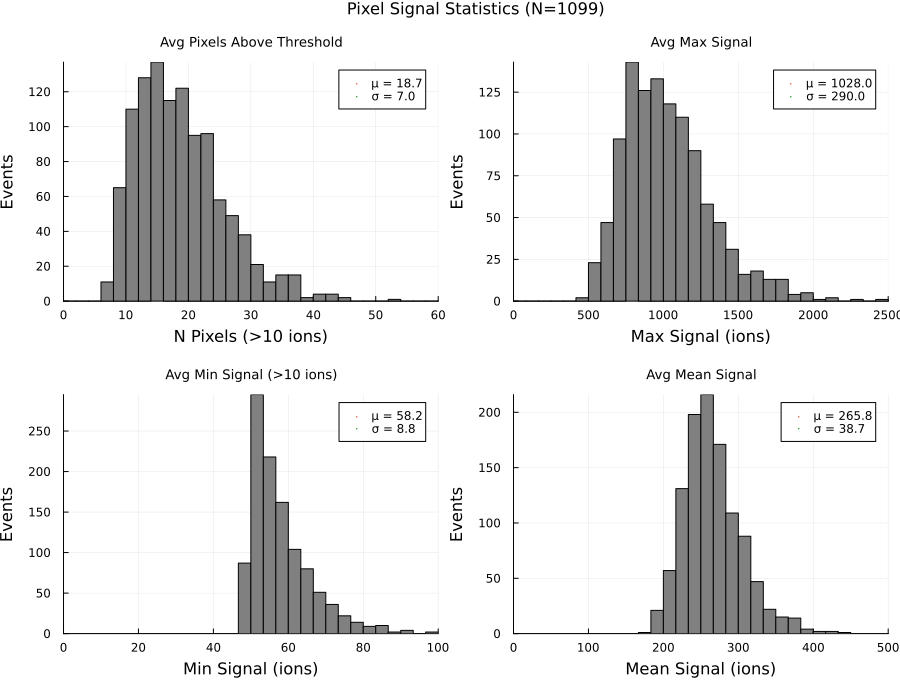
\includegraphics[scale=0.40]{img/single_track_pixel_signals.png}
%     \caption{Top-left panel: number of pixels per frame;  top-right: average number of ions
% per pixel and frame; bottom-left: minimum number of ions per pixel and frame;
% bottom-right: maximum number of ions per pixel and frame. Simulation conditions as in Table \ref{tab:itaca_params} (15 bar, 200 V/cm, Xe${^2+}$ ions,
%   thermal diffusion of eq. \eqref{eq:drift}), applied to the \bbonu\ sample of
%   Section~5.2 of Ref.~\cite{itaca2026} (N = 1099 events).
% }
% \label{fig:px}
% \end{figure}
% 
% A \bbonu\ event (or a single electron in the ROI) produces $\sim 10^5$ ions, distributed in about
% $\sim 20$ pixels per frame (Figure~\ref{fig:px}, top-left panel). The average number of ions
% per pixel and frame is $\sim 260$ (Figure~\ref{fig:px}, top-right panel). The minimum signal above threshold (which we take as 10 ions) is $\sim 58$ on average and always above $\sim 45$ ions (Figure~\ref{fig:px}, bottom-left panel). The maximum signal is $\sim 1028$ ions on average and practically never exceeds 2500 (Figure~\ref{fig:px} bottom-right panel). 
%     
% 
% The target equivalent noise charge for the NAUSICA front-end is
% \begin{equation}
%     \mathrm{ENC} \sim 50~e^{-} \ \mathrm{RMS},
% \end{equation}
% which gives $S/N \sim 5$ for the average pixel signal and keeps the minimum signal at the level of the noise; this target is 3.5 times looser than the noise demonstrated by Topmetal-II~\cite{An2016TopmetalII}. 
% 
% The dynamic range is modest and amply covered with the standard CMOS ADC of 12 bits. 
% 
% \subsubsection*{Readout architecture and digitisation}
% 
% The detector is read out using a frame-based scan of all pixels. For an $80 \times 80$ pixel
% array, corresponding to 6400 pixels, a frame period of 10~ms implies an aggregate sampling
% rate of
% $
%     6.4 \times 10^5~\mathrm{samples\,s^{-1}}.
% $
% Digitization is implemented at the periphery of the ASIC or on an external carrier, using
% one or a small number of multiplexed ADCs. A resolution of 12 bits over a full-scale range
% of approximately 1~V provides quantisation noise well below the analogue noise level.
% 
% \subsubsection*{Die size and tiling strategy}
% 
% Given the large pixel pitch, only a modest number of pixels can be accommodated per die.
% A baseline design adopts dies of approximately
% $
%     20 \times 20~\mathrm{mm^2},
% $
% each hosting a $10 \times 10$ pixel matrix. This results in 100 pixels per die.
% 
% A full $80 \times 80$ pixel detection plane is obtained by tiling $8 \times 8 = 64$ such dies
% on a common carrier, yielding a contiguous active area of
% $16 \times 16~\mathrm{cm^2}$. All periphery and I/O structures are oriented outward, ensuring
% that no inactive regions are introduced within the sensitive area.
% 
% 
% 
% END ORIGINAL SECTION 3

\section{Scope and definitions}


The carrier is the molecular ion \ion, containing two xenon atoms but carrying
one positive elementary charge, $q=e=1.602176634\times10^{-19}$ C. 
A \bbonu\ event produces around $10^5$ ions which carry 16.02 fC, before any collection loss.

The readout pad is at $z=0$ and positive $z$ points upward into the gas. Positive
ions move toward decreasing $z$. ``Current'' means the equivalent source
current delivered into the pad's readout input, with positive sign for a positive
ion approaching the selected pad. 

This stage assumes fixed electrode potentials,
negligible perturbation of the drift field by the ion charge, a linear dielectric
response and negligible conducting response of the gas or substrate on the
timescale of interest. These assumptions permit the static weighting-field
description. 


\section{Detector definition and revised voltages}
The geometry and bulk operating point are based on the design discussion and
the ITACA context~\cite{itaca2026}. The revised IFG voltages were supplied in the
design discussion and supersede the voltage scheme in that preprint. Table~\ref{tab:inputs}
identifies assumptions that still need experimental or engineering confirmation.

\begin{table}[ht]
\centering\small
\begin{tabular}{llp{5.6cm}}
\toprule
Parameter & Value & Status \\
\midrule
Ion charge & $+e$ & Molecular $\mathrm{Xe}_2^+$ assumption \\
Pressure & 15 bar & Detector design \\
Temperature & 293.15 K & Room-temperature benchmark \\
Bulk reference length & 1.5 m & Reference drift; not track length \\
Bulk drift speed & 0.1 m/s & Operating assumption, not a mobility measurement \\
Hole diameter / pitch & 0.5 / 2 mm & Circular holes on a square pitch \\
IFG thickness / pad gap & 10 / 5 mm & Revised geometry \\
Pad width & 0.5 mm & Square used for analytical benchmark; outline to confirm \\
\bottomrule
\end{tabular}

\caption{Inputs to the first benchmark. The complete numerical definition and
provenance are in \texttt{config/detector.toml}.}
\label{tab:inputs}
\end{table}

\begin{figure}[ht]
\centering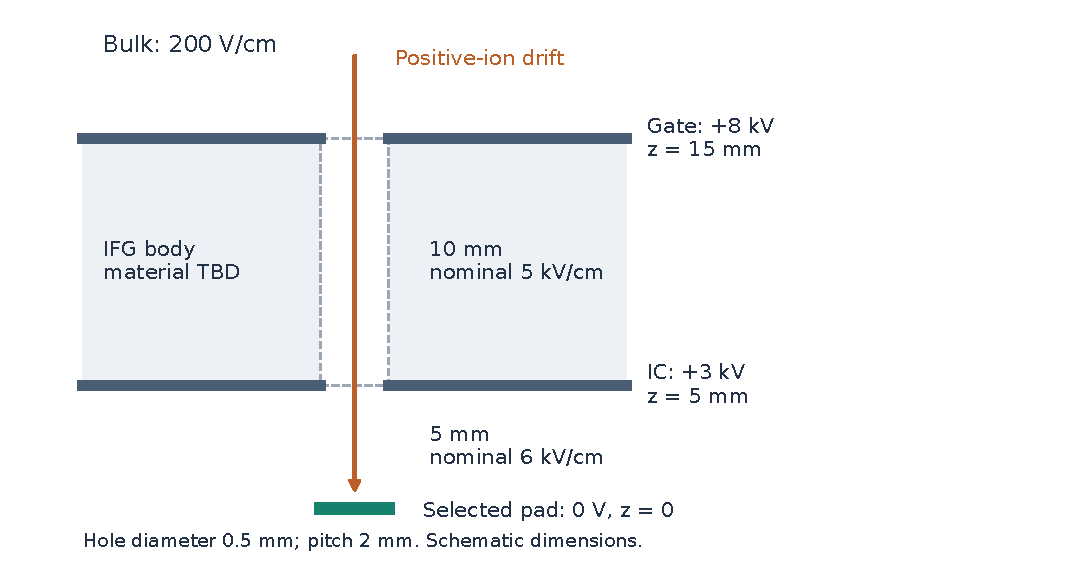
\includegraphics[width=.94\linewidth]{geometry.pdf}
\caption{Local coordinate and voltage convention. The hole walls and IFG body
are schematic; their material and electrical treatment remain unresolved.
The drawing does not represent a solved electric field.}
\label{fig:geometry}
\end{figure}

With the pad at zero, the IC is at $+3$ kV and the gate at $+8$ kV. The nominal
potential gradients are
\begin{equation}
 E_{\rm h}=\frac{8-3\ \mathrm{kV}}{10\ \mathrm{mm}}
 =5\ \mathrm{kV/cm},\qquad
 E_{\rm g}=\frac{3\ \mathrm{kV}}{5\ \mathrm{mm}}
 =6\ \mathrm{kV/cm}.
\end{equation}
These are field magnitudes; the axial physical electric field points downward.
Within and around real apertures the field is nonuniform. Dividing a voltage
drop by a distance supplies a nominal scale, not an aperture-field solution.

\clearpage
\subsection{Focusing must be checked at the entrance}
For circular holes of diameter $d_h$ on a square pitch $p$, the open fraction is
\begin{equation}
 f=\frac{\pi(d_h/2)^2}{p^2}=\OpenFraction.
\end{equation}
If all electric flux through one drift-region cell is to pass through its hole,
the simplified flux budget requires
\begin{equation}
 E_{\rm h} A_h\gtrsim E_{\rm d}p^2,
 \qquad E_{\rm h}\gtrsim\frac{E_{\rm d}}{f}
 =\EntranceThreshold\ \mathrm{kV/cm}.
 \label{eq:focus}
\end{equation}
Here the incident field is the \emph{bulk} field, $E_{\rm d}=200$ V/cm. Applying
this check at a different interface would miss the entrance bottleneck. The
nominal revised design gives $fE_{\rm h}/E_{\rm d}=\FluxRatio$, above unity.

Equation~\eqref{eq:focus} is a flux-capacity check under a simplified cell model.
It does not establish unit ion transparency. Field lines can terminate on grid
metal, diffusion can carry ions into walls, and material boundaries and alignment
can alter the collection map. The larger downstream nominal field supports
confinement of the exiting flux; it does not prove that every exiting ion lands
on the intended metal pad.

\section{Nominal transport and diffusion}
\subsection{Mobility inferred from the bulk operating point}
The working drift law is $v=\mu E$. The stated bulk speed implies
\begin{equation}
 \mu=\frac{0.1\ \mathrm{m/s}}{2.0\times10^4\ \mathrm{V/m}}
 =\Mobility\times10^{-6}\ \mathrm{m^2/(V\,s)}
 =0.05\ \mathrm{cm^2/(V\,s)}.
\end{equation}
This is the mobility at the working gas density; it is not the reduced mobility
normalized to a reference pressure. Extrapolating it unchanged to the IFG and
gap is an explicit approximation. The assumption must be checked against
mobility data over the relevant reduced-field range.

\begin{table}[ht]
\centering\small
\begin{tabular}{lrrrr}
\toprule
Region & $E$ (kV/cm) & $E/p$ (kV/cm/bar) & $v$ (m/s) & $t$ (ms) \\
\midrule
Bulk reference & 0.2 & 0.0133 & 0.1 & 15000.000 \\
IFG hole & 5 & 0.3333 & 2.5 & 4.000 \\
Collection gap & 6 & 0.4000 & 3 & 1.667 \\
\bottomrule
\end{tabular}

\caption{Uniform-field estimates using the same mobility in each region.
Reduced fields use the design pressure of 15 bar. The bulk reference path is
1.5 m, whereas the hole and gap paths are 10 and 5 mm respectively.}
\label{tab:regions}
\end{table}

The nominal IFG and gap transit times are therefore 4.0 and 1.67 ms. Their sum
is a common final-transport delay for otherwise identical trajectories. Neither
this sum nor the 15 s full bulk drift is the duration of a single-pad current
pulse. The pulse duration also depends on where the pad weighting potential
changes along the trajectory.

\clearpage
\subsection{Thermal diffusion as a reference model}
In the thermal, isotropic limit, the Einstein relation gives
\begin{equation}
 D=\frac{\mu k_BT}{e}=\DiffusionCoefficient\times10^{-7}\ \mathrm{m^2/s}.
\end{equation}
For a uniform drift distance $L$, the one-coordinate RMS spatial spread is
\begin{equation}
 \sigma=\sqrt{2Dt_d}
       =\sqrt{\frac{2k_BT}{e}\frac{L}{E}},\qquad t_d=\frac{L}{v}.
 \label{eq:diffusion}
\end{equation}
The thermal transverse form is also used in the ITACA design discussion
\cite{itaca2026}. Here $\sigma$ denotes one Cartesian coordinate, not the
two-dimensional radial RMS, which would be $\sqrt{2}\sigma$ for an isotropic
Gaussian. Taking the same coefficient longitudinally is an additional
thermal-isotropy assumption.

For one-dimensional constant drift and diffusion toward an absorbing plane,
the first-passage-time distribution has mean $L/v$ and variance $2DL/v^3$.
Equivalently, its RMS time spread is
\begin{equation}
 \sigma_t=\frac{\sigma_L}{v}.
 \label{eq:time_spread}
\end{equation}
The distribution is well approximated by a Gaussian when its relative width
is small. These formulas describe bulk transport; they are not a prescription
for transporting a covariance matrix through a nonuniform focusing field.

\begin{table}[ht]
\centering
\begin{tabular}{rrrr}
\toprule
$L$ (m) & $t_d$ (s) & $\sigma$ (mm) & $\sigma_t$ (ms) \\
\midrule
0.1 & 1 & 0.503 & 5.026 \\
0.75 & 7.5 & 1.376 & 13.765 \\
1.5 & 15 & 1.947 & 19.466 \\
\bottomrule
\end{tabular}

\caption{Thermal bulk-diffusion benchmark at 293.15 K and 200 V/cm. The arrival
time spread uses the bulk speed of 0.1 m/s.}
\end{table}

\begin{figure}[ht]
\centering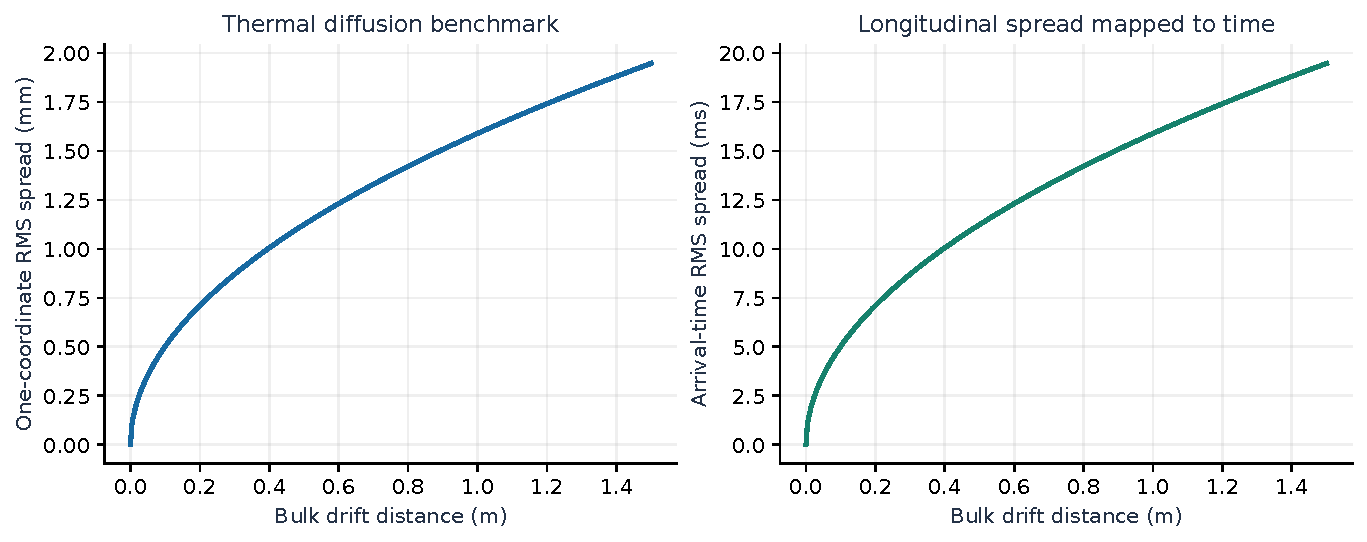
\includegraphics[width=\linewidth]{transport.pdf}
\caption{Spatial and temporal diffusion scales before the IFG. These are
calculated reference values, not measurements of ion transport.}
\end{figure}

A millimetre of longitudinal spread corresponds to 10 ms of arrival-time spread
at the bulk drift speed. Applying the faster gap velocity to that upstream
spread would incorrectly compress the arrival interval: ions entering the
same final trajectory at different times retain that time separation. The
focusing map and additional diffusion in the final regions require trajectory
transport to be treated quantitatively.

\clearpage
\section{Weighting potential and the single-ion signal}
\subsection{Two distinct electrostatic problems}
The physical potential $V$ determines ion trajectories through
$\mathbf E=-\nabla V$ and, in this approximation, $\mathbf v=\mu\mathbf E$.
It uses the actual electrode voltages. The weighting potential $\phi_w$ for one
readout pad instead satisfies
\begin{equation}
 \nabla\!\cdot\!\bigl(\epsilon(\mathbf r)\nabla\phi_w\bigr)=0,
 \qquad
 \phi_w=\begin{cases}1&\text{selected pad},\\0&\text{all other fixed-potential electrodes}.
 \end{cases}
 \label{eq:weighting}
\end{equation}
The ion is removed from this auxiliary problem. Dielectric interfaces obey
continuity of potential and of normal displacement in the absence of an imposed
free surface charge. Geometry, materials and boundary conditions determine
$\phi_w$; changing the applied biases alone does not change this weighting
potential. Floating or resistive electrodes would require a more general
treatment~\cite{riegler2016,riegler2019}.

With $\mathbf E_w=-\nabla\phi_w$ and our current convention,
\begin{align}
 i_p(t)&=q\frac{\dd\phi_w(\mathbf r(t))}{\dd t}
       =-q\,\mathbf v(t)\cdot\mathbf E_w(\mathbf r(t)),\label{eq:ramo}\\
 \int_{t_a}^{t_b}i_p(t)\,\dd t
       &=q\left[\phi_w(\mathbf r(t_b))-\phi_w(\mathbf r(t_a))\right].
       \label{eq:charge}
\end{align}
In this normalization $\phi_w$ is dimensionless and $\mathbf E_w$ has units
of inverse length. An ion starting where $\phi_w$ is negligible and reaching
the selected pad therefore gives an integrated signal of approximately $e$.
Neighboring pads can have transient induced currents even if they do not
collect the ion; their net signal is zero when both endpoint weighting
potentials are zero.

The ion induces current while approaching the electrode. After collection
its macroscopic drift contribution ceases. A separate extra charge-$e$ impulse
at impact would double count the charge already included in
Eq.~\eqref{eq:charge}. Microscopic surface processes are outside this model.

\subsection{What the focusing grid changes}
The fixed-potential grid screens the pad's weighting potential in the upstream
volume, with leakage through its apertures. The extent of that screening must
be calculated for the actual structure. This note does not assume an exact zero
weighting potential above a perforated grid. The current near a small pad is
generally not described by $qv/d$ with the full chamber drift length $d$.
That familiar expression follows from a uniform weighting field between broad
parallel electrodes, for which $\phi_w$ varies linearly across their separation.

The use of electrostatics is a quasistatic approximation. A light-propagation
time $d/c$ is not an ion-current rise time in this model; the waveform is set
by charge motion through the weighting field.

\clearpage
\section{Analytical central-pad benchmark}
\subsection{Boundary conditions and derivation}
Consider a square pad of side $2a$ in the plane $z=0$, set to unit weighting
potential. The remainder of that infinite plane is a grounded conductor. The
upper half-space is a homogeneous dielectric, with potential tending to zero
at infinity. This replaces the real IFG and dielectric stack by a tractable
reference boundary-value problem.

The half-space Poisson kernel gives~\cite{salazar2021}
\begin{equation}
 \phi_w(x,y,z)=\frac{1}{2\pi}\int_{-a}^{a}\!\int_{-a}^{a}
 \frac{z\,\dd x'\,\dd y'}{[(x-x')^2+(y-y')^2+z^2]^{3/2}}.
 \label{eq:poisson}
\end{equation}
It is the solid angle subtended by the pad divided by $2\pi$. Evaluating the
integral on the central axis yields
\begin{equation}
 \boxed{\phi_w(z)=\frac{2}{\pi}\tan^{-1}
 \left[\frac{a^2}{z\sqrt{z^2+2a^2}}\right]},\qquad z>0,
 \label{eq:square_phi}
\end{equation}
with the limiting value $\phi_w(0)=1$. Its positive normal weighting field is
\begin{equation}
 W(z)=-\frac{\dd\phi_w}{\dd z}
 =\frac{4a^2}{\pi(z^2+a^2)\sqrt{z^2+2a^2}}.
 \label{eq:square_field}
\end{equation}
The implemented formula is independently compared with numerical evaluation
of Eq.~\eqref{eq:poisson}. At large $z$, $\phi_w\simeq2a^2/(\pi z^2)$ and
$W\simeq4a^2/(\pi z^3)$; the pad response is concentrated near the metal.

For a central normal trajectory at constant speed $v$, let collection occur
at $t=0$. Then $z=-vt$ before collection and
\begin{equation}
 i_1(t)=\begin{cases} ev\,W(-vt),&t<0,\\0,&t\geq0.\end{cases}
 \label{eq:pulse}
\end{equation}
The one-sided value immediately before collection is
\begin{equation}
 i_1(0^-)=\frac{2\sqrt{2}}{\pi}\frac{ev}{a}.
\end{equation}
The step to zero idealizes collection at the metal and infinite readout
bandwidth. The smooth approach is a drift-averaged current; it does not resolve
individual gas collisions or atomic-scale image-force dynamics.

The pulse scales as $i_{\rm peak}\propto v/a$ and duration $\propto a/v$, while
its full integrated charge is $e$. The same constant-speed benchmark extended
to $t=-\infty$ has a mathematically integrable tail. That extension must not be
interpreted as the real trajectory through the upstream grid.

\clearpage
\subsection{Numbers, duration definitions and finite-path charge}
Using $a=\SquareHalfWidth$ mm and $v=\GapSpeed$ m/s gives the results in
Table~\ref{tab:pulse}. To define charge-based durations, invert the potential:
\begin{equation}
 z(\phi)=a\sqrt{\frac{1}{\sin(\pi\phi/2)}-1}.
\end{equation}
The cumulative full-path signal fraction before collection is $\phi_w(z)$.
The final interval containing fraction $F$ of the signal has duration
$z(1-F)/v$. The central 90\% interval instead runs from cumulative fractions
0.05 to 0.95. These durations differ from the time above half peak; none is an
exponential decay constant.

\begin{table}[ht]
\centering\small
\begin{tabular}{lr}
\toprule
Quantity & Value \\
\midrule
Peak immediately before collection & 1.731 fA \\
Characteristic time $a/v$ & 83.33 $\mu$s \\
Time above half peak & 70.52 $\mu$s \\
Final interval containing 90\% of charge & 193.51 $\mu$s \\
Final interval containing 99\% of charge & 659.67 $\mu$s \\
Central 90\% interval (5--95\%) & 280.96 $\mu$s \\
Cumulative charge 10--90\% rise & 184.21 $\mu$s \\
Charge induced from 5 mm to the metal & 0.9984124 $e$ \\
\bottomrule
\end{tabular}

\caption{Central square-pad benchmark. Full-path fractional durations refer to
the ideal half-space model, without electronic shaping.}
\label{tab:pulse}
\end{table}

\begin{figure}[ht]
\centering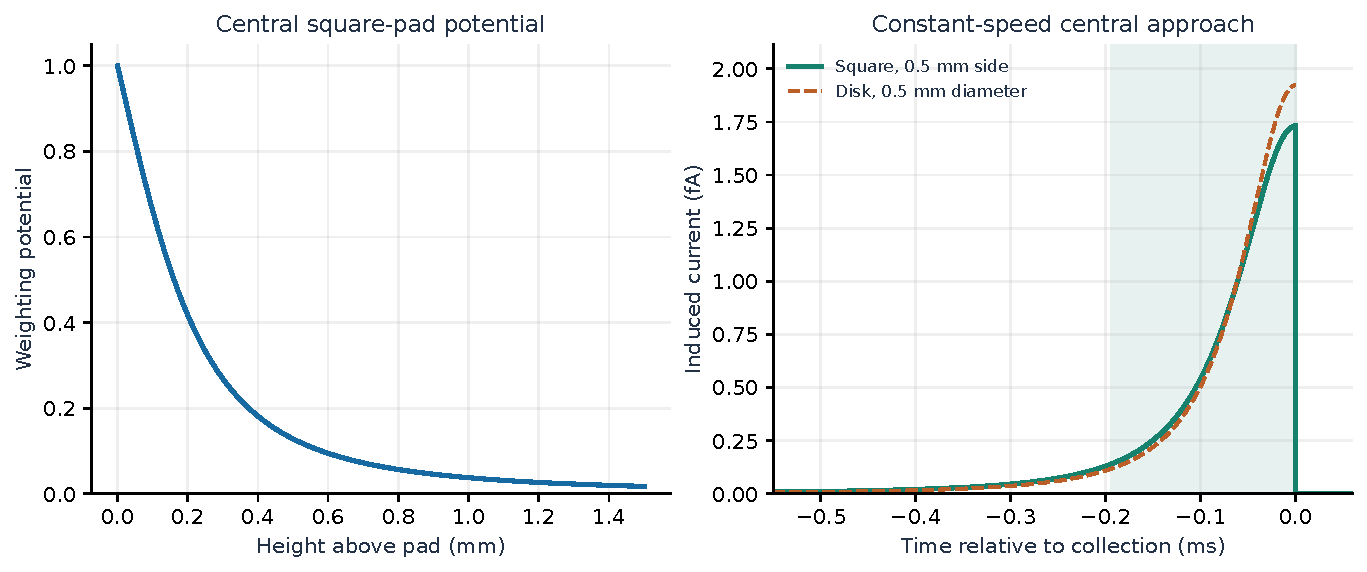
\includegraphics[width=\linewidth]{single_ion.pdf}
\caption{Analytical weighting potential and current. The shaded interval
contains the final 90\% of the square-pad signal. The circular-pad comparison
uses the same grounded-plane assumption and the same lateral diameter as the
square side. The physical geometry is not resolved by either model.}
\end{figure}

For a trajectory beginning at the nominal gap height $g=5$ mm,
\begin{equation}
 \phi_w(g)=\GapPotential,\qquad
 Q_{g\to0}=e[1-\phi_w(g)]=\GapChargeFraction\,e.
\end{equation}
The missing \GapMissingPercent\% belongs to the earlier part of this idealized
trajectory. It is not discarded or reassigned by normalization. A full IFG
solution will distribute the entire signal according to its own weighting
potential and trajectory. Small $\phi_w(g)$ in this model does not bound the
error from different pad surroundings or dielectric boundaries.

\clearpage
\subsection{Geometry dependence and an independent shape comparison}
For a circular pad of radius $a$ in the same infinite grounded plane, direct
integration of the Poisson kernel gives
\begin{equation}
 \phi_{w,\circ}(z)=1-\frac{z}{\sqrt{z^2+a^2}},\qquad
 W_\circ(z)=\frac{a^2}{(z^2+a^2)^{3/2}}.
\end{equation}
Its central peak is $ev/a=\DiskPeakCurrent$ fA for diameter 0.5 mm, compared
with \PeakCurrent\ fA for the 0.5 mm square. This difference is a comparison
of two specified boundary problems, not a systematic uncertainty estimate for
the actual pad. Off-centre trajectories and ideal sharp edges can change the
local peak appreciably; finite electrode edges, gaps and dielectrics matter.

\begin{table}[ht]
\centering
\begin{tabular}{rrr}
\toprule
$z$ (mm) & $\phi_w(z)$ & $i(z)$ (fA) \\
\midrule
5 & 0.001588 & 0.000304 \\
1 & 0.037470 & 0.033940 \\
0.5 & 0.128188 & 0.199874 \\
0.25 & 0.333333 & 0.706661 \\
0.1 & 0.661663 & 1.435876 \\
0.05 & 0.822863 & 1.647985 \\
0 & 1.000000 & 1.730959 \\
\bottomrule
\end{tabular}

\caption{Square-pad sensitivity and central current at selected heights. The
row at $z=0$ gives the pre-collection limit, not the current after absorption.}
\end{table}

An unknown region between pads cannot be assigned a zero weighting potential
merely because neighboring pads are at zero in the auxiliary problem. A
grounded metal plane enforces a Dirichlet boundary; an exposed dielectric
requires a dielectric-interface solution. This distinction is likely more
important than the square-versus-disk comparison. The present benchmark has
no quantitative uncertainty envelope for that missing geometry.

\section{Implications for the next physics stage}
The ion trajectory takes milliseconds through the last structures, while the
central benchmark induces most of its pad signal in a fraction of a millisecond.
Bulk diffusion can spread arrivals over tens of milliseconds. These are three
different timescales. A many-ion input is the sum of the appropriate single-ion
signals, each placed at its own collection time.

For a curved event, depth orders arrival time. Total electron path length does
not fix the time span on one pad. The 10 cm straight segment aligned with drift
is retained only as a diagnostic extreme. Realistic calculations must preserve
the event's isotropic orientation, scattering, nonuniform deposition, endpoint
blobs and repeated intersections with a pad's collection region.

\clearpage
\section{Validation, reproduction and remaining work}
The automated suite contains independent physical checks:
\begin{enumerate}
\item The nominal voltage drops and region lengths reproduce the revised fields.
\item The thermal spread agrees with both $\sqrt{2Dt}$ and the uniform-drift
first-passage time variance.
\item Numerical surface integration reproduces the square-pad potential.
\item A finite-difference derivative reproduces the analytical weighting field;
surface and far-field limits and monotonicity are checked.
\item Independent quadrature gives unit full-path weighting-field integral,
and the finite-gap integral equals its endpoint potential difference.
\item Velocity scaling preserves charge and stretches time inversely; sampled
spatial integration converges as its step is reduced.
\end{enumerate}
Passing these checks establishes implementation consistency. It does not
measure ion transparency, real drift coefficients, or the actual ASIC response.

From the repository root, the reproducible entry points are
\begin{verbatim}
make PYTHON=<python-with-dependencies> test physics
make PYTHON=<python-with-dependencies> note
\end{verbatim}
The scripts read \texttt{config/detector.toml}; numerical results and environment
versions are saved in \texttt{results/physics\_benchmarks.json}. This note
includes generated figures, tables and value macros. The configuration hash
prefix for the present build is \texttt{\ConfigHash}. The analytical model is
deterministic and has no random seed.

Before replacing the benchmarks with a detector prediction, establish the pad
outline, surrounding metallization and guard electrodes; the IFG wall material
and metallization; the dielectric stack; and alignment and edge geometry.
Obtain or justify mobility and longitudinal/transverse diffusion over the
operating reduced fields. Solve the physical and weighting fields separately,
checking domain and mesh convergence and integral charge identities.

The next stage will map three-dimensional energy deposits into pad-specific
arrival distributions, then into current waveforms. Packet charge, central-90\%
duration, peak current, repeated-packet separation and charge per readout bin
will form the interface to the electronics study. Feedback-retention
requirements and the properties of Rogelio's feedback transistor remain outside
the scope of this note.

\bibliographystyle{unsrtnat}
\bibliography{references}
\end{document}
